%/*****************************************************************************
% *
% * $Id: CMakeLists.txt 2392 2013-05-03 18:22:41Z kyle.shannon $
% *
% * Project:  WindNinja
% * Purpose:  DEM download instructions.
% * Author:   Kyle Shannon <kyle@pobox.com>
% *
% *****************************************************************************
% *
% * THIS SOFTWARE WAS DEVELOPED AT THE ROCKY MOUNTAIN RESEARCH STATION (RMRS)
% * MISSOULA FIRE SCIENCES LABORATORY BY EMPLOYEES OF THE FEDERAL GOVERNMENT
% * IN THE COURSE OF THEIR OFFICIAL DUTIES. PURSUANT TO TITLE 17 SECTION 105
% * OF THE UNITED STATES CODE, THIS SOFTWARE IS NOT SUBJECT TO COPYRIGHT
% * PROTECTION AND IS IN THE PUBLIC DOMAIN. RMRS MISSOULA FIRE SCIENCES
% * LABORATORY ASSUMES NO RESPONSIBILITY WHATSOEVER FOR ITS USE BY OTHER
% * PARTIES,  AND MAKES NO GUARANTEES, EXPRESSED OR IMPLIED, ABOUT ITS QUALITY,
% * RELIABILITY, OR ANY OTHER CHARACTERISTIC.
% *
% * THE SOFTWARE IS PROVIDED "AS IS", WITHOUT WARRANTY OF ANY KIND, EXPRESS
% * OR IMPLIED, INCLUDING BUT NOT LIMITED TO THE WARRANTIES OF MERCHANTABILITY,
% * FITNESS FOR A PARTICULAR PURPOSE AND NONINFRINGEMENT. IN NO EVENT SHALL
% * THE AUTHORS OR COPYRIGHT HOLDERS BE LIABLE FOR ANY CLAIM, DAMAGES OR OTHER
% * LIABILITY, WHETHER IN AN ACTION OF CONTRACT, TORT OR OTHERWISE, ARISING
% * FROM, OUT OF OR IN CONNECTION WITH THE SOFTWARE OR THE USE OR OTHER
% * DEALINGS IN THE SOFTWARE.
% *
% ****************************************************************************/

\documentclass[12pt,oneside,final]{article}
\title{How to download an elevation file using WindNinja}
\author{Cody Posey}
\date{\today}
\usepackage[margin=0.75in]{geometry}
\usepackage{graphicx}
\usepackage{hyperref}

\begin{document}

\maketitle

\begin{figure}[ht!]
    \centering
    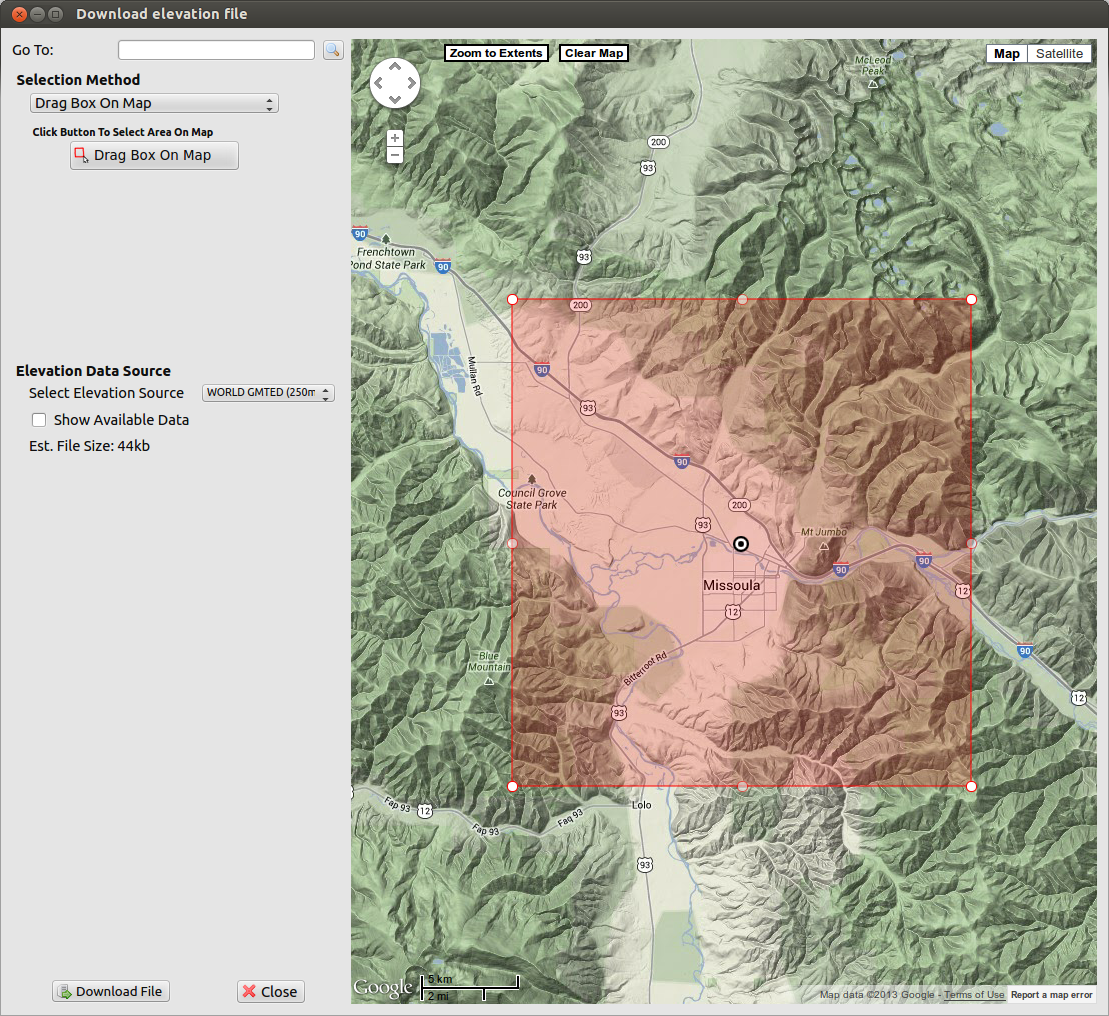
\includegraphics[width=7in]{images/download_dem_0.png}
    \caption{fetch\_dem help message}
    %\label{overflow}
\end{figure}

\section{Introduction}

This document describes the functionality built into WindNinja to download
elevation files for wind modeling.  We call this utility the “elevation file
grabber”.  It allows you to use a custom Google Mapsä interface to zoom into
and select a desired area for wind modeling. The elevation data for this area
is downloaded by WindNinja from a USGS server and saved to a file on your
computer.  There is also a command line version of the elevation file grabber
that is described \href{run:./fetch_dem_instructions.pdf}{here}.  The specific
options available and work flow are described below.

To open the elevation file grabber window, start WindNinja and click Surface
Input in the navigation tree at the top of WindNinja, then click the Download
File button as shown below.

\begin{figure}[ht!]
    \centering
    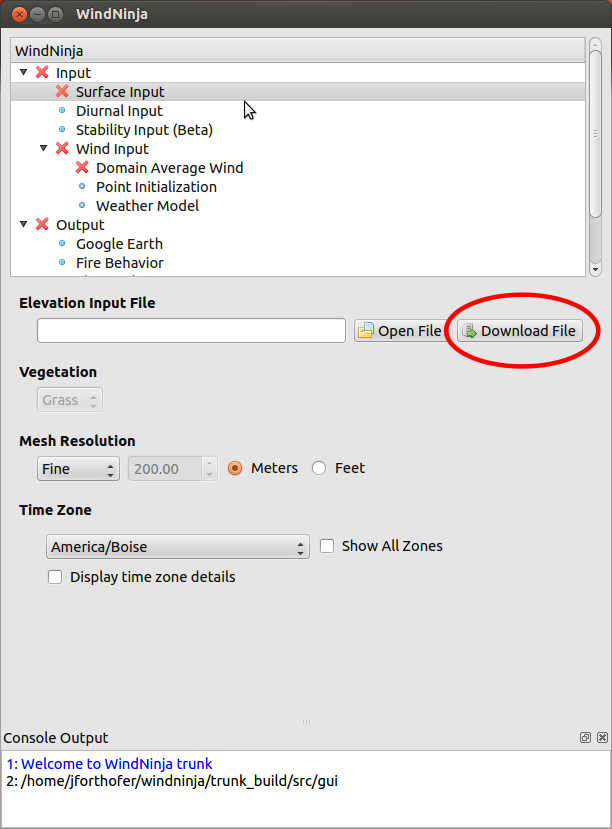
\includegraphics[width=5in]{images/download_dem_1.png}
    \caption{fetch\_dem help message}
    %\label{overflow}
\end{figure}

The Download Elevation File window will open.  This window is divided into two
areas as highlighted in red in the image below.  These areas are discussed in
the next two sections.

\begin{figure}[ht!]
    \centering
    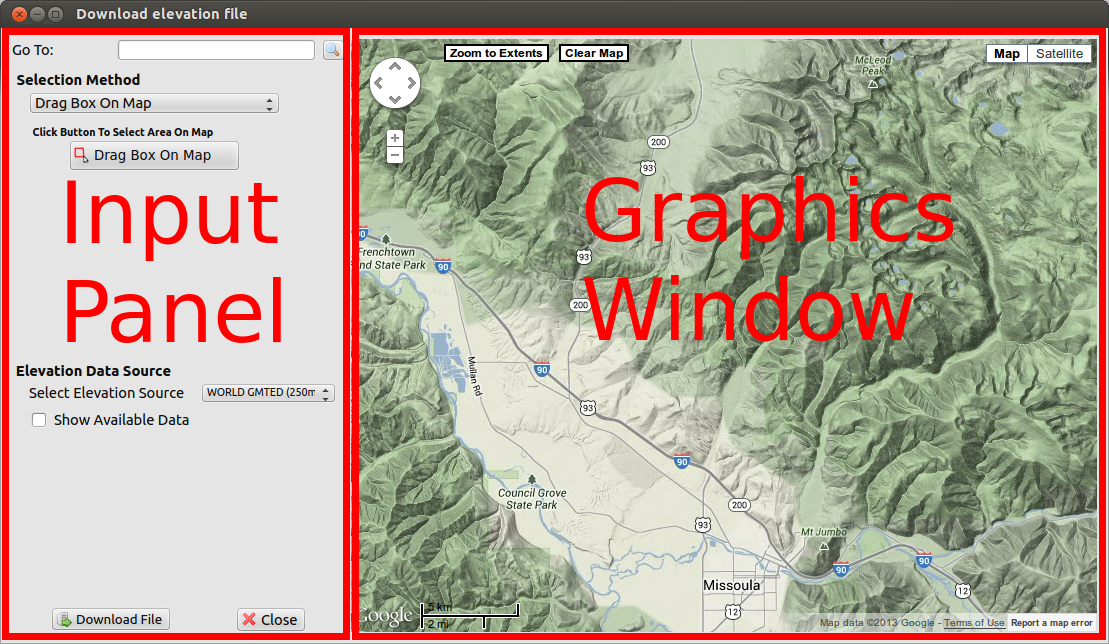
\includegraphics[width=7in]{images/download_dem_2.png}
    \caption{fetch\_dem help message}
    %\label{overflow}
\end{figure}

\section{Graphics Window}

The graphics window is an interactive mapping display used to navigate into the
desired wind simulation area.  This window uses a customized version of the
popular Google MapsÔ software.  Various different base maps are available using
the 'Map' and 'Satellite' buttons in the upper right corner.  There are several
ways to pan and zoom the map.  Using a mouse, you can pan with the left button
and zoom using a mouse scroll wheel.  You can also left-click the navigation
controls in the upper left corner of the graphics window.  Last, the keyboard
can be used to pan (arrow keys) and zoom (plus and minus keys).

\section{Input Panel}

\subsection{Zoom to geographic location}

At the top of the panel, there is a 'Go To:' text box where you can type in
geographic locations to quickly zoom to.  Some example searches are: “Missoula,
MT”, “Pikes Peak, CO”, and “Redfish Lake, ID”.

\subsection{Download area selection method}

Below the 'Go To:' text box is the Selection Method group of buttons and text
boxes that allow you to define the area you want to download.  This download
area is a rectangular box that will be drawn over the map in the graphics
window.  There are four different ways to define this rectangular box that can
be chosen from the drop-down box.  They are:

\begin{itemize}
    \item{Drag Box On Map}
        By clicking the Drag Box On Map button, you can then left-click and
        drag on the graphics window to define a box of the desired size.
    \item{Enter Bounding Box}
        This option allows you to enter the latitude and longitude bounds for
        the box.
    \item{Click Center Point}
        This option allows you to click a center point on the map to define the
        center of the box and then enter the size of the box.
    \item{Enter Center Point}
        With this method, you enter the center point coordinates of the box and
        the box size.  After using any of the methods above, a transparent red
        box will be drawn in the graphics window showing the area you've
        defined.  If you want, you can enlarge or shrink this box in the
        graphics window by dragging the sides or corners.  You can also move
        the box by dragging the center icon.  The Zoom To Extents button in the
        graphics window will zoom the view to fit the box. The Clear Map button
        will clear the box.
\end{itemize}

\section{Elevation data source}

There are 3 possible online data sets to download elevation data from.  These
are listed in the Select Elevation Source drop-down box.  The main difference
between these data sets is the spatial resolution and extent.  The table below
briefly describes these differences.  You should be sure to choose a data set
that covers your simulation area.

\begin{center}
    \begin{tabular}{| l | l | p{1.75in} | p{1.75in} |}
    \hline
    Data set name & Resolution & Spatial Extent & Description \\ \hline

    US SRTM & 30 meters  & Contiguous US, Hawaii, PR, Southern Alaska &
    Data from the Shuttle Radar Tomography Mission (SRTM) \\ \hline

    WORLD SRTM & 90 meters & Between approximately -60 and +60 latitude &
    Data from the Shuttle Radar Tomography Mission (SRTM) \\ \hline

    WORLD GMTED & 250 meters & Between approximately -60 and +85 latitude &
    Global Multi-resolution Terrain Elevation Data 2010 (GMTED 2010) \\ \hline

    Landscape (LCP) & 30 meters & Contiguous US, Hawaii, PR, Southern Alaska &
    FarSITE Landscape files including vegetion information \\ \hline
\end{tabular}
\end{center}

\noindent
You can check the Show Available Data check-box to display a blue polygon on
the map outlining the chosen data set's extents.

\section{Download the file}

Once you have defined your download area and selected the elevation data
source, click the Download File button at the bottom to download the elevation
file.  A window will open to allow you to specify a file name and location.
The downloaded file is a geotiff file (*.tif) in a best fit UTM projection and
a WGS84 datum.  After the file is successfully downloaded, you can close the
Download elevation file window and the downloaded file will be automatically
loaded into the main WindNinja window.

\end{document}

